\chapter{Solar irradiance simulation tools}
The primary tool used in this thesis for simulating PV generation with different parameters is the python library PVlib. PVlib contains be built functions for estimating solar irradiance, angle of incidence and a multitude of other useful tools. As seen in Table \ref{table_poa_simulated_format}, the plane of array(POA) simulations which estimate the irradiance per 1m² of solar panel surface resemble the earlier FMI PV datasets in their structure.

%An example of the irradiance simulation outputs is shown in table \ref{table_poa_simulated_format} and the table shows that the output format is simular to the FMI PV datasets shown earlier in table \ref{table_fmi_kumpula_csv}.




%Having a mathematical model which would simulate the output of a PV system would allow for the parameters of a PV installation to be solved with model fitting. In the best case scenario, we would have a physics based model which would take geographic location, panel installation angles, time of year and panel surface area or power rating as inputs and the output would be similar to the data from FMI Kumpula installation seen in table \ref{table_fmi_kumpula_csv}. Creating a such model is rather challenging as the model has to take into account atmospheric scattering, Sun angles, Sun-Earth distance variation and a multitude of other factors, the consideration of which are far beyond this mathematics thesis. Luckily the modeling of the energy output of solar PV installations has uses for the cost-benefit analysis of solar PV installations and thus pre-existing modeling algorithms are publicly available. 


% TODO REWRITE

%This thesis uses a plane of array irradiance simulation function from the python library PVlib. The function takes geographic location, timestamp and panel angles as inputs. The outputs contain power values which describe the amount of direct and atmospherically scattered light that would hit a square meter sized imaginary solar panel with the input parameters. The sum of these sources is referred as plane of array (POA) irradiance and this value can be used to estimate the output of solar power installations. A section of simulated data is included in table \ref{table_poa_simulated_format}.

%As the model simulates radiation values during clear sky conditions and not the power output of pv installations, the model should be seen as an approximation which is accurate to a certain degree. The differences between the model and recorded measurements could be due to reflectivity of the solar panels, weather conditions, temperature related changes in efficiency, atmospheric composition or a multitude of other factors which the model does not take into account.

\begin{table}[h]

\centering

\begin{tabular}{r|cccc} \hline\hline

Timestamp[UTC] & Minute & POA(W) \\ \hline
$2018-05-30$ $00:00$ &  $0$ & $0.0$\\
$2018-05-30$ $00:01$ &  $1$ & $0.0$\\
$2018-05-30$ $00:02$ &  $2$ & $0.0$\\
\vdots & \vdots & \vdots \\
$2018-05-30$ $ 07:34$ & $454$ & $800.691861$\\
$2018-05-30 $ $07:35$ & $455$ & $802.110516$\\
$2018-05-30 $ $07:36$ & $456$ & $803.517424$\\
\vdots & \vdots & \vdots \\
$2018-05-30$ $ 23:57$ & $1437$ & $0.0$\\
$2018-05-30 $ $23:58$ & $1438$ & $0.0$\\
$2018-05-30 $ $23:59$ & $1439$ & $0.0$\\

\hline\hline
\end{tabular}
\tabcaption{One day of simulated plane of array irradiance values. Note that the minute column is added to the table for convinience and it is reduntant as minutes can be read from the timestamps.}
\label{table_poa_simulated_format}
\end{table}


\subsection{PVlib POA function inputs} 
%PVlib plane of array irradiance can be simulated with 

%\begin{lstlisting}[caption={PVlib POA simulation function header.}, label={poa_header}]
%def get_irradiance(year, day, lattitude, longitude, tilt, azimuth):
%\end{lstlisting}


\noindent The following listing contains the relevant parameters of the plane of array irradiance function and their domains.
%The POA simulation function accepts real --or integer as is the case with the day parameter-- valued parameters in the ranges listed below. 

\begin{itemize}
	\item Year $\in \mathbb{N}$
	\item Day [1, 365/366] $\in \mathbb{N}$
	\item Latitude [-90, 90] $\in \mathbb{R}$%, Finland fits within subrange [59, 70]
	\item Longitude [-180, 180]  $\in \mathbb{R}$%, Finland fits within subrange [19, 32] 
  	\item Tilt [0, 90] $\in \mathbb{R}$
  	\item Azimuth [0, 360[ $\in \mathbb{R}$
\end{itemize}

%\noindent \textbf{Note:} While the function does accept the full latitude and longitude ranges as inputs, it may be beneficial to restrict the range of the coordinate parameters when the approximate location of the installation is known. For example, Finland fits within subrange [19, 32] on the longitude axis and thus it could make sense to restrict the longitude range when examining installations located within Finland.

\vspace{3mm}
\noindent
The day and year parameters can be assumed to be always known as datasets include timestamps and this leaves four unknown system parameters. These four parameters span a 4D parameter space of possible PV installations. The size of this parameter space is connected to the difficulty of the parameter estimation problem. As the parameters are in $\mathbb{R}$, the amount of sensible combinations is the product of the discretization of each of the parameter ranges. Tilt and azimuth parameters can be discretized as integers, resulting in $90*360$ or $32400$ unique angle space points. The geographic latitude and longitude coordinates are somewhat harder to discretize. In an arbitrary 0.1 degree geographic discretization there would be $1800*3600$ or 6480000 coordinate combinations. The product of these two sums results in $2*10^{11}$ unique parameter combinations.

A parameter space this large is difficult to examine exhaustively. Even a system capable of evaluating 100 000 angle space points per second would need approximately 23 days in order to evaluate all of the possible combinations. However if the parameters can be solved in isolation from oneanother, the required computational time would decrease significantly. Instead of $90*360*1800*36000$, there would be $90+360+1800+3600$ combinations to evaluate. This highlights how important it is to break problems into smaller pieces whenever possible and much of this thesis focuses on how this can be done with solar PV parameter estimation. 


\newpage
\section{PVlib POA evaluation}

Before implementing the parameter estimation functions, the POA simulations should be tested against known measurement data. Figure \ref{fig-multidaypoavsmeasurements} displays that in clear sky conditions the pvlib irradiance model is following real world measurements closely with a few exceptions. And during cloudy days the measurements are often lower than the clear sky model would indicate, but they can also peak higher than they would during cloud free days. These increases of power generation above clear sky estimated power are likely to be caused by the additional sunlight reflected from clouds towards solar panels in partly cloudy weather conditions and it shows that cloud induced noise can be positive as well as negative. 



\begin{figure}[h]
\centering
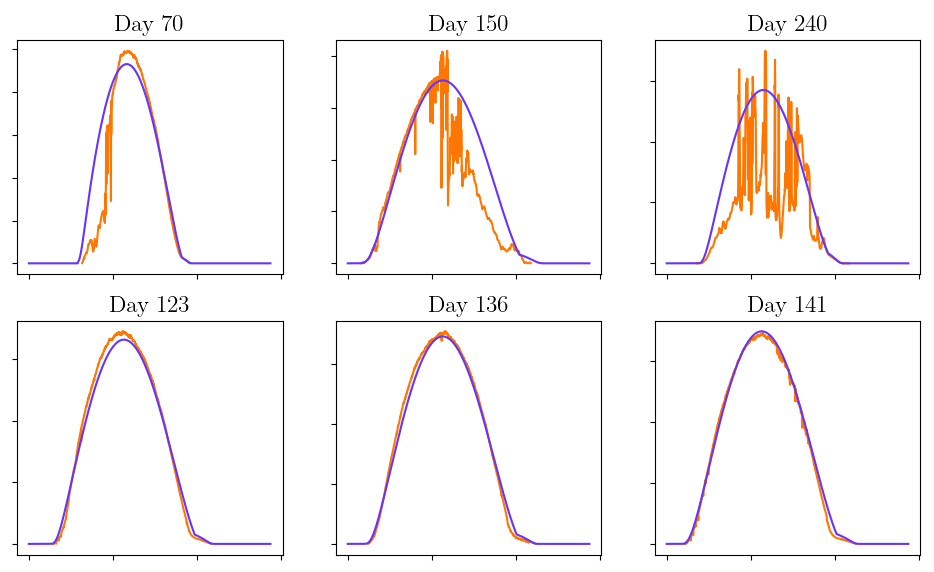
\includegraphics[width=0.9\linewidth]{pics/multiday_vs_neat}
\figcaption{Power output of FMI Kumpula PV installation and the pvlib POA simulation computed with the parameters from Table  \ref{table_fmi_helsinki_kuopio_parameters}. Horizontal axis on the graphs corresponds to time and vertical axis marks the estimated power values. The purpose of the graphs is to display the different shapes and deviations from POA models and thus axis names and numbers were left out. Upper row contains randomly selected days while as the lower row has days chosen by a clear sky algorithm mentioned in Chapter \ref{clearskyalgo_chapter}. Measurements are from 2017. POA irradiance values were multiplied by 19 in order to match the curves values on power axis.}
\label{fig-multidaypoavsmeasurements}
\end{figure}



% On the 70th and 150th day, the first and last minutes do not seem to be exactly the same as in the simulation, but the difference seems minor and it is occuring in different directions.






%\textit{The following claims are unverified conjectures, but the smooth shape and the early date of the first graph could hint that the increased peak production on the 70th day could be due to reflections from snow, while as the more irregular production on the 150th and 240th day would seem to indicate that the variation is caused by clouds. Filtering out days such as the 150th or the 240th from the dataset should be rather simple as the high frequency component is noticeable, but low frequency deviations such as the smooth increase in production of the 70th day could prove to be more difficult to detect algorithmicly.}






\newpage
%\section{Influence of different parameters on the PVlib poa model}
%\label{influence_parameters}



\begin{figure}[ht!]
\centering
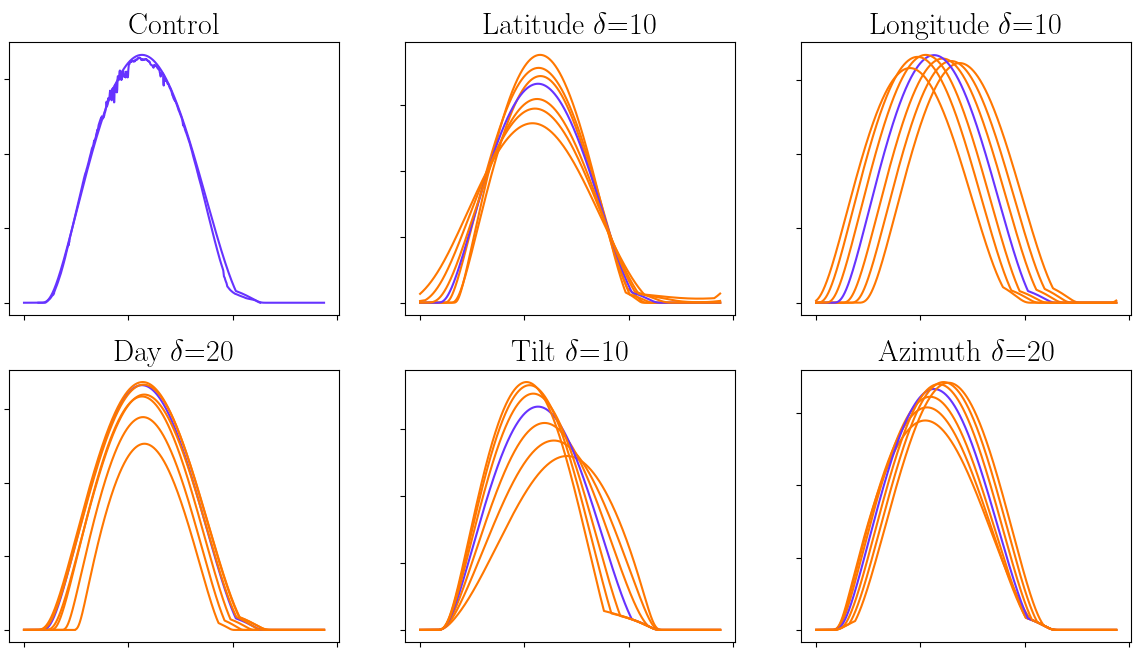
\includegraphics[width=0.9\linewidth]{pics/poa_eval_new_crop}
\figcaption{Influence of changes in PVlib simulation parameters on generated power output curves. Control shows FMI Helsinki measurements and simulation with the same parameters as the Helsinki installation. Simulated power values are multiplied by 19 in order to match values on y-axis.}
\label{fig_poa_different_parameters}
\end{figure}

\noindent By varying the different simulation parameters as shown in Figure \ref{fig_poa_different_parameters}, we can examine the relationships between parameters and power generation curves. This can help us understand if there are usable patterns in the data. In the best case scenario each of the simulation function inputs would affect one measureable property in the irradiance plots and their relationship would be bijective. To give an example, if the peak power minute was isolated from all other parameters than the longitude and the relationship between longitude and peak power minute was linear, it would be possible to solve the peak power minute to longitude function with just a few plane of array irradiance simulations.

In the exact opposite case where every measureable property of irradiance plots is affected by every input parameter, solving the parameters would be much harder or even impossible. For example if all of the parameters influenced the same traits to different extents and the system was not bijective, multiple parameter combinations could result in the same simulated power graph. In a such system there would not be a single solution but rather a set of possible solutions.

The problem of solving installation parameters would appear to be somewhere in between the two extremes. The longitude parameter would seem to shift the curve along the time axis where as tilt and azimuth parameters do not affect the first or last non-zero minutes but they do affect the shape of the curve. Observations of parameter to trait interactions are listed on Table \ref{table_traits}.



\begin{table}[H]
\centering
\begin{tabular}{r|cc} \hline\hline

 Parameter & Traits affected\\ \hline
 Latitude & Shape, first and last minute times\\
 Longitude & First and last minute times\\
 Tilt & Shape\\
 Azimuth & Shape\\

\hline\hline
\end{tabular}
\tabcaption{Function input to observed trait table.}
\label{table_traits}
\end{table}


%Base on these observations, the relationship between longitude and the First and last minute times would seem like the best starting point for parameter solving.

%If the POA model is assumed to be accurate, the model could be used to simulate the effects of different parameters on power generation. This could provide insights into the relationship between patterns in the data and the parameters of the system. The relevant parameters to simulate and their default values can be seen in table \ref{table_default_parameters_poa_simulations}. In the following simulations, only one of the default parameters is varied. This is done in order to isolate the effect of individual parameters.



%\begin{table}[!ht]
%\centering
%\begin{tabular}{r|c} \hline\hline

% Parameter & Value \\ \hline
% Day & $180$  \\
% Latitude & $60^\circ$  \\
% Longitude & $28^\circ$  \\
% Panel tilt & $30^\circ$ \\
% Panel angle & $180^\circ$  \\
%\hline\hline
%\end{tabular}
%\tabcaption{Default parameters for POA simulation used in this section. }
%\label{table_default_parameters_poa_simulations}
%\end{table}


\newpage

\subsection{Influence of different longitudes}
\label{section_different_longitudes}

\begin{figure}[ht!]
\centering
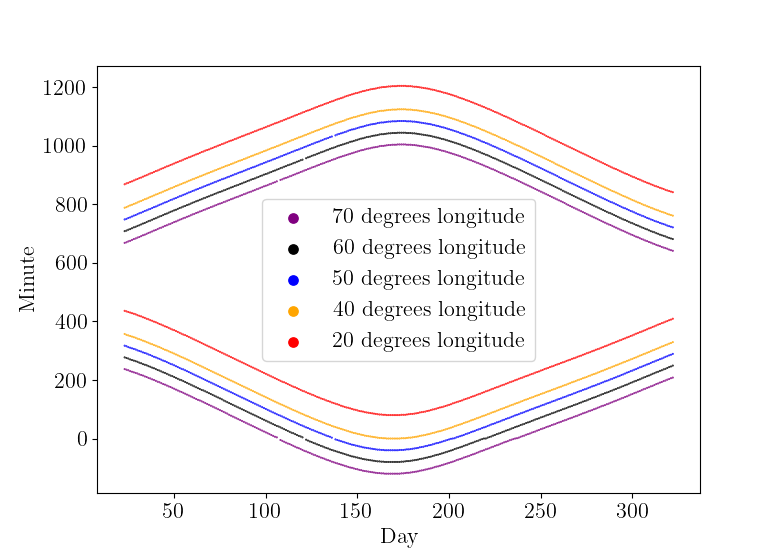
\includegraphics[width=1\linewidth]{pics/poa_var_lon}
\figcaption{First and last non-zero minutes of each day from year long simulations at different longitudes.}
\label{fig-poa_var_lon2}
\end{figure}

\noindent Based on earlier observations listed in Table \ref{table_traits}, solving the longitude of installations would seem like a sensible starting point. The figure comparing the effects of different parameters seemed to suggest that the relationship between longitude and significant minute times is very close to linear and the same is seen here in Figure \ref{fig-poa_var_lon2}. In Hagdadi 2017 \cite{navid_australian_article} and in Williams 2012 \cite{older_solar_solver_article} this relationship was used in order to determine the geographic longitude. The algorithms used by both of the articles relies on calculating an approximation for the time of the solar noon based on the average of the first and last minutes, this solar noon minute is then translated into a geographic longitude coordinate.





%There are at least two ways of estimating the longitude from the UTC solar noon time. First method is based on fitting a linear equation to a list of known solar noon to longitude-pairs. This would result in an equation of the form $f(x) = 0.25^\circ* x + b$ where the solar noon minute $x$ is multiplied by the constant $0.25$. The constant of $0.25^\circ$ comes from dividing a full circle by the amount of minutes in a day, 1440. The constant $b$ is around $-180^\circ$ and it is the result of solar noon occuring close to noon.
%In the figure \ref{fig-poa_var_lon2}, the relationship between the first and last minutes of a day and the geographic longitude can be seen to be linear. This linear equation should be of the form $f(x) = 0.25^\circ* x + b$ where the solar noon minute $x$ is multiplied by the constant $0.25$. The constant of$0.25^\circ$ comes from dividing a full circle by the amount of minutes in a day, 1440. The constant $b$ is roughly $-180$ degrees as that is the offset required for adjusting solar noon from



%and the figure \ref{fig-poa_var_lon2} it would seem that the relationship between longitudes and first and last minutes is a good starting point for parameter so


%at least very close to linear. In Hagdadi 2017 \cite{navid_australian_article} and in Williams 2012 \cite{older_solar_solver_article} this relationship was used in order to determine the geographic longitude. The algorithms used by both of the articles relies on calculating an approximation for the time of the solar noon based on the average of the first and last minutes, this solar noon minute is then translated into a geographic longitude coordinate.

% and a similar algorithm is detailed in []..




\newpage

\subsection{Influence of different latitudes}
\label{section_different_latitudes}

\begin{figure}[ht!]
\centering
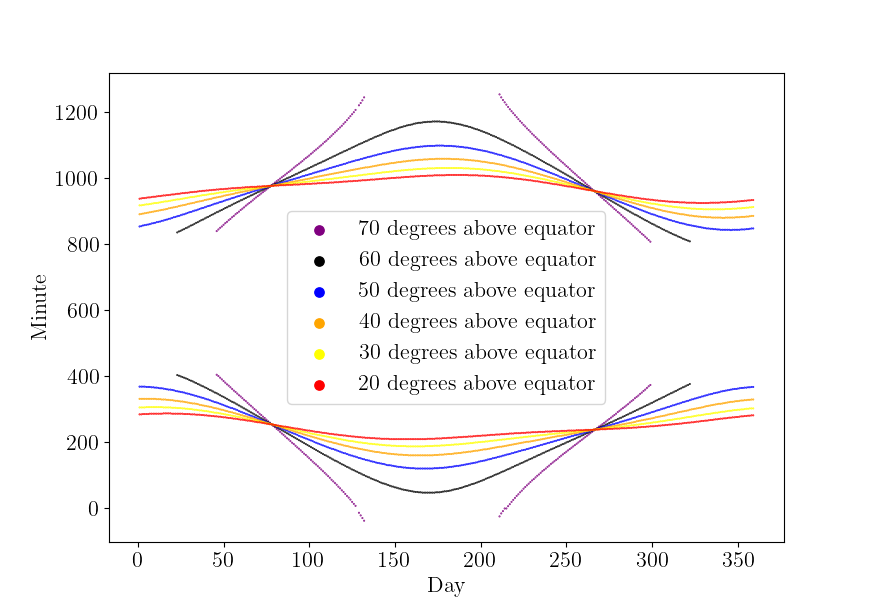
\includegraphics[width=1\linewidth]{pics/poa_var_lat}
\figcaption{First and last non-zero power minutes of each day from year long simulations at different latitudes}
\label{fig_poa_var_lat}
\end{figure}

\noindent The latitude simulations in Figure \ref{fig_poa_var_lat} show that the day length stays fairly consistent for locations close to the equator, but with latitudes of $50^\circ$ and higher, the day to day variation is significant. These POA simulations would imply that the region around equinoxes is ideal for day length based analysis as there day length is always well defined and the rate of change can be measured. 


\newpage

\section{Increasing the accuracy of solar PV simulations}
\label{section_increased_accuracy_simulations}


\begin{figure}[h]
\centering
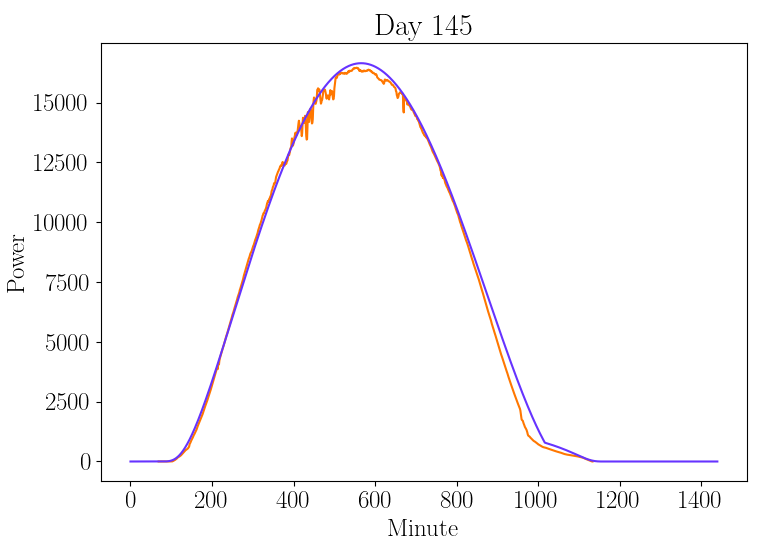
\includegraphics[width=0.7\linewidth]{pics/poa_eval_single_day}
\figcaption{Figure comparing Pvlib simulated POA irradiance and actual measured PV output of FMI Helsinki installation.}
\label{fig-poa_eval_single_day}
\end{figure}

\noindent Figure \ref{fig-poa_eval_single_day} compares the simulated and measured PV output during a sunny day in Helsinki. The shapes of the curves match quite closely, but there are some discrepancies. The estimated power values for the peak production hours are higher than measured power values and a similar phenomena is seen near minute 1000. These discrepancies can be explained by real world phenomena as PVlib POA values describe the amount of radiation reaching the surface of a solar panel. This is different from the power output of a PV system as thermal losses and panel reflections are not taken into account. This section examines an improved PV model which includes these losses.

\newpage

\subsection{Improved PV model}

\begin{figure}[h]
\centering
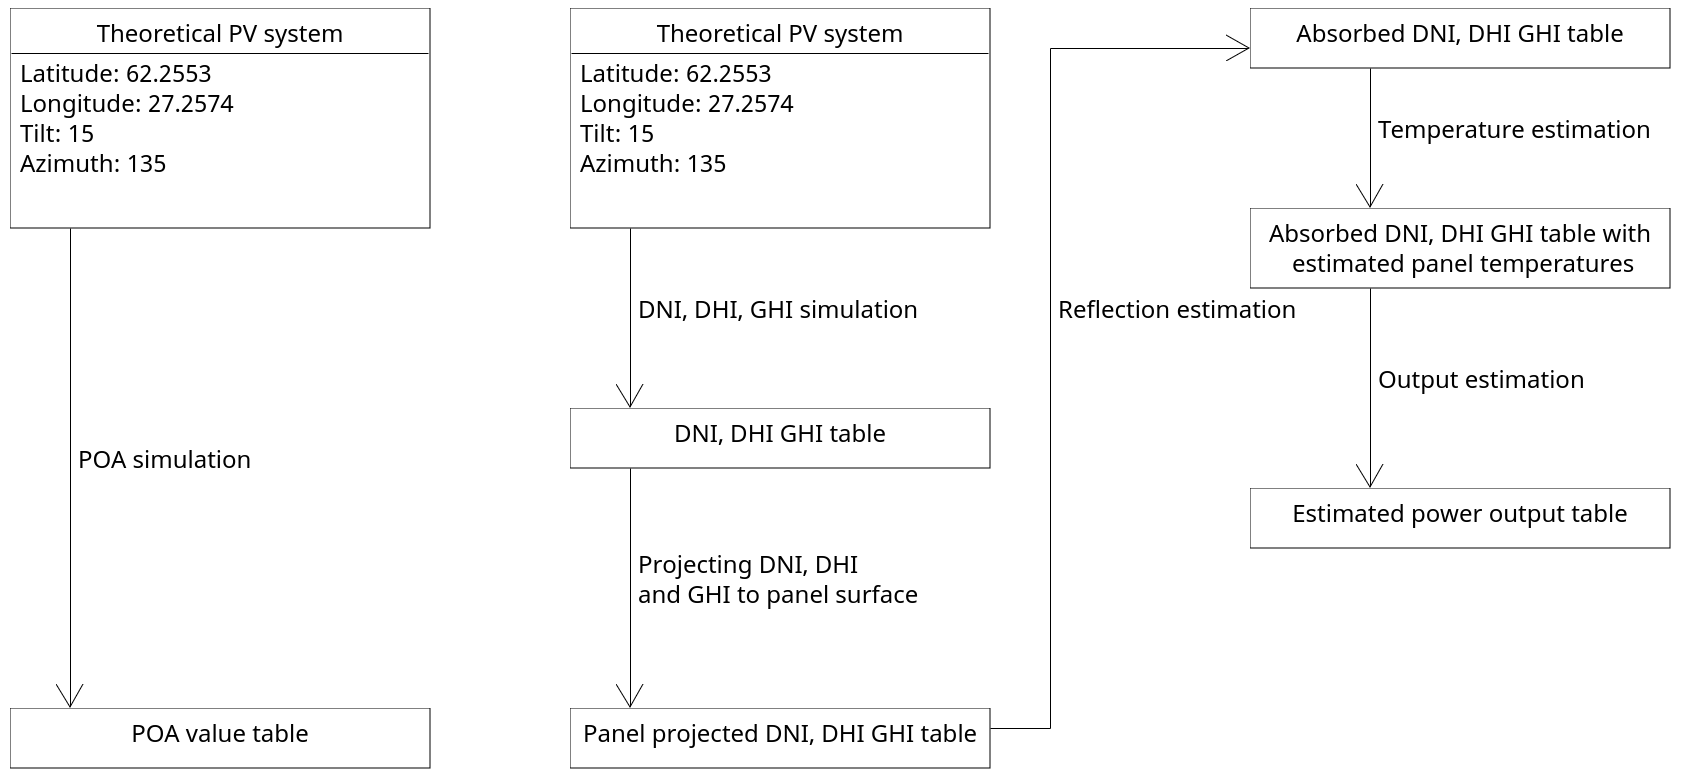
\includegraphics[width=1.0\linewidth]{pics/uml2}
%\captionsetup{labelformat=empty}
\figcaption{Original POA-based PV model and the improved model with reflection and temperature estimation.}
\label{fig-pv_model}
\end{figure}


\noindent 
The improved PV model in Figure \ref{fig-pv_model} introduces some new concepts, among which are the following irradiance types.

\begin{itemize}
\item DNI is diffused normal irradiance which represents direct sunlight received by a 1m² -sized plane with AOI of 0 degrees. Note that athmosphere scattered or ground reflected irradiance are not components of DNI.

\item DHI is diffuse horizontal irradiance which represents the irradiance reaching a shaded 1m² -sized plane with tilt of 0 degrees. DHI represents atmosphere scattered irradiance.

\item GHI is global horizontal irradiance and it represents the amount of irradiance per 1m² -sized plane with tilt of 0 degrees. GHI is made up of direct irradiance and atmosphere scattered irradiance. GHI combined with albedo can be used to estimate the ground reflected irradiance.
\end{itemize}

\noindent
These irradiance types are present in both the simpler PVlib POA based model and the improved PV model. The difference between the two models is that in the POA-model, PVlib internally calculates three irradiance components DNI, DHI and GHI and projects them to the panel surface, returning the resulting sum as plane of array irradiance. Where as in the more complex PV model, PVlib estimates DNI, DHI and GHI, each of which are processed by multiple functions before they are combined into an estimated power output value, resulting in a physically more accurate PV output estimation.

\subsection{Panel surface projections}

The first step in the improved model is panel surface projection. Sandia National Laboratories, the original author of PVlib, suggests the following two equations for DNI and GHI projection and five alternative models for DHI projection. Perez 1990 model \cite{perez} was chosen for DHI projections due to the use of the model by a co-worker at FMI and inclusion in Sandia suggested projection models \cite{sandia_poa_dhi}. For implementation of DNI, DHI and GHI equations, see thesis source code.

%As there are three irradiance types with different apparent sources and thus directions, three irradiance projection functions are needed. The simplest way to project DNI and DHI to panel surface is to use the equations $DNI_{proj}= DNI* sin(AOI)$ and $DHI_{proj}= DHI* sin(tilt)$ both of which are mathematically trivial. However ground reflected irradiance projection is not as simple. The original author of PVlib, Sandia National Laboratories recommends the use the following two equations for DNI and GHI, offering five different models for DHI. 


\noindent\textbf{DNI projection}\cite{sandia_poa_dni}
%
\begin{equation}
\begin{split}
\label{sandia_eq_dni}
DNI_{proj}(DNI, AOI)= DNI*cos(AOI)
\end{split}
\end{equation}
Where $AOI$ is the angle of incidence.


\noindent\textbf{GHI projection}\cite{sandia_poa_ghi}
%
\begin{equation}
\begin{split}
\label{sandia_eq_ghi}
GHI_{proj}(GHI, albedo, tilt)= GHI*albedo*\frac{1-cos(tilt)}{2}
\end{split}
\end{equation}

\noindent Where 

%\noindent 
$albedo = 0.151$. This represents ground reflectivity near the solar PV installation. The value varies significantly depending on the area, season and time of day. A fixed value is used as terrain, weather and snow cover are assumed to be unknown.

%\noindent 
$tilt$ is the tilt angle of the PV installation, this is $15^\circ$ for both FMI installations.

%\noindent\textbf{DHI projection}\cite{sandia_poa_dhi}
%\begin{equation}
%\begin{split}
%\label{sandia_eq_dni}
%GHI_{proj}(DHI, tilt) = See source
%\end{split}
%\end{equation}

\newpage
\subsection{Reflection estimation and absorbed irradiance}
The following Solar irradiance reflection equations originate from 2001 Martin and Ruiz paper \cite{solar_reflections}. This study used a physical contraption in which solar panels were rotated under a light beam from a solar simulator. Values from the reflective losses equations represent the fraction of irradiance reflected away from the panels e.q. a $DNI_{reflected}$ value of 0.24 would tell us that 24\% of irradiance is lost due to reflections and 76\% is absorbed. 

\noindent\textbf{DNI reflective lossess}

% THIS IS F_A(Beta) in original source
\begin{equation} 
\begin{split}
\label{solar_reflecive_dni_loss} 
DNI_{reflected}= exp(-\frac{1}{a_r}(c_1 p_1 +c_2 p_1^2))
\end{split}
\end{equation}


% THIS IS F_D(Beta) in original source
\noindent\textbf{DHI reflective lossess}
%
\begin{equation}
\begin{split}
\label{solar_reflecive_dhi_loss}
DHI_{reflected}= exp(-\frac{1}{a_r}(c_1 p_2 +c_2 p_2^2))
\end{split}
\end{equation}

\noindent\textbf{GHI reflective lossess}
%
\begin{equation}
\begin{split}
\label{solar_reflecive_ghi_loss}
GHI_{reflected} = \frac{exp(-cos(\alpha)/a_r)- exp(-1/a_r)}{1-exp(-1/\alpha_r)}
\end{split}
\end{equation}

\noindent Where

$a_r = 0.159$ Empirical reflectance constant for polycrystalline silicon solar PV panels.

$c_1= \frac{4}{3\pi}$  Fitting parameter 1.

$c_2 = -0.074$ Fitting parameter 2.

$p_1= sin(tilt) + \frac{tilt-sin(tilt)}{1-cos(tilt)}$

$p_2= sin(tilt) + \frac{\pi - tilt-sin(tilt)}{1+cos(tilt)}$


\noindent\textbf{Absorbed irradiance}
\begin{equation}
\begin{split}
\label{solar_reflecive_absorbed}
POA_{absorbed} = DNI(1-DNI_{r})+ DHI(1-DHI_{r})+GHI(1-GHI_{r})
\end{split}
\end{equation}

\noindent Where $DNI$, $DHI$ and $GHI$ are solar irradiance values in watts and $DNI_r$, $DHI_r$, $GHI_r$ refer to Equation \ref{solar_reflecive_dni_loss}, \ref{solar_reflecive_dhi_loss} and \ref{solar_reflecive_ghi_loss}.





\subsection{Panel temperature estimation}
Panel temperatures need to be estimated as the efficiency of solar panels depends on panel temperature. This can be accomplished with the following King et al 2004 model\cite{king2004} if air temperature, wind speed and absorbed radiation are known. Note that as the model does not take the thermal capacity of the panels into account, the actual panel temperature is likely smoother and delayed compared to modeled temperature.

\noindent\textbf{Panel temperature}
\begin{equation}
\begin{split}
\label{panel_temp}
T_{panel} = T_{air} + POA_{absorbed} e ^{C_a+ C_b*w}
\end{split}
\end{equation}

\noindent Where 

$T_{air}$ is air temperature in $^\circ C$.

$C_a = -3.47$ Model fitting constant.

$C_b = -0.0594$ Model fitting constant. 

$w$ is wind speed at panel elevation.


\vspace{6mm}

\noindent As air temperature and wind speed are unknown, dummy values have to be used for both variables. Air temperatures of 20$^\circ C$ and wind speed of 2m/s were used as dummy values.

\newpage
\subsection{Output estimation}
Now that the absorbed radiation and panel temperature are known, the output can be estimated with the following Huld et al 2010 model\cite{huld2010}.

\noindent\textbf{PV output model}
\begin{equation}
\begin{split}
\label{pv_output_model}
P_{output} = P_{rated}  P_n  \eta_{rel}
\end{split}
\end{equation}

\noindent Where 

$P_{rated}$ is the rated power of the system in kW.

$P_n = \frac{POA_{absorbed}}{1000}$

%$POA_{absorbed}$ is \ref{solar_reflecive_absorbed}.

$\eta_{rel}= 1+k_1 ln(P_n) + k_2 ln(P_n)^2 + T_{diff}k_3 + k_4 ln(P_n) + k_5 ln(P_n)^2 + k_6 T_{diff}^2$

In $\eta_{rel}$ the variables $k_1$ to $k_6$ are fitting parameters and $T_{diff}$ is $T_{panel}-25^\circ C$.

\begin{table}[h]
\begin{tabular}{l|l|l|l|l|l}
k1        & k2        & k3        & k4       & k5       & k6       \\ \hline
-0.017162 & -0.040289 & -0.004681 & 0.000148 & 0.000169 & 0.000005
\end{tabular}
\end{table}

\noindent %This leaves the rated power of the system as an unknown parameter. 
For unknown PV systems, the unknown value $P_{rated}$ can be estimated with the following area matching equation \ref{pv_area_matching}. Note that as the sum of $P_{simulated}$ varies depending on installation angles and geolocation, the multiplier value has to be calculated every time an unique set of PV system parameters is simulated. Visualization of area matching is shown in Figure \ref{fig_area_match}.


%This is the process of calculating the integral or sum of power generation plots and matching their values. A 1kW system can be matched. Visualization of this process where a POA simulation of a 1kW installation is area matched with known measurement data is shown in Figure \ref{fig_area_match}.


\noindent\textbf{Area matching}
\begin{equation}
\begin{split}
\label{pv_area_matching}
Multiplier = \sum_{t=0}^{1439} P_{measured}(t)/ \sum_{t=0}^{1439} P_{simulated}(t)
\end{split}
\end{equation}

\noindent Where

$P_{simulated}$ is simulated output of a 1kW installation.

$Multiplier$ is an approximation of $P_{rated}$ and the accuracy of the approximation increases as parameters used for $P_{simulated}$ near the parameters of the unknown PV installation.



%by comparing the sum of measured power output values to the sum of simulated power output with a theoretical 1kW system. Visualization of this process with POA simulations and real measurements is shown in Figure\ref{fig_area_match}.


\begin{figure}[h]
\centering
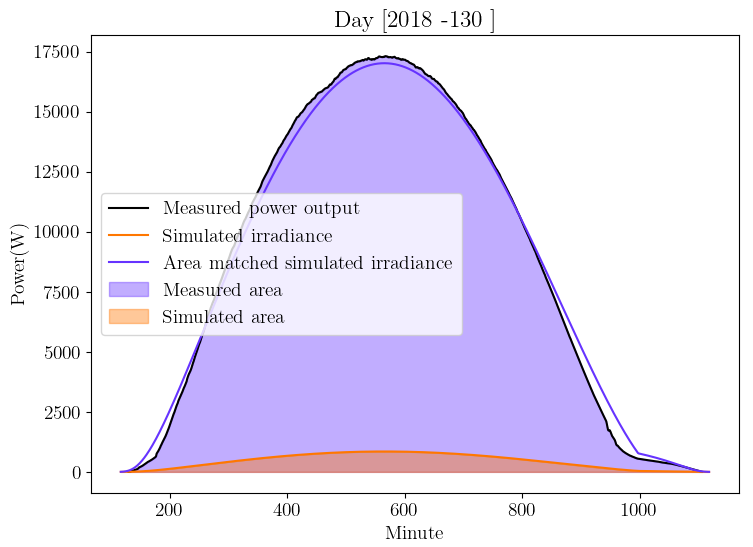
\includegraphics[width=0.7\linewidth]{pics/areamatching2}
\figcaption{Measurement data from FMI Helsinki dataset, POA irradiance simulation was computed with FMI Kumpula coordinates and installation angle parameters.}
\label{fig_area_match}
\end{figure}

\newpage
\subsection{Model improvement results}
The models can be compared with the original measurement data with the following Equation \ref{pv_model_delta}.



\noindent\textbf{Model delta}
\begin{equation}
\begin{split}
\label{pv_model_delta}
Delta_{model} = \sum_{t=0}^{1439} |P_{measured}(t) - P_{simulated}(t)| /1440
\end{split}
\end{equation}

\noindent The delta value represents a normalized per minute deviation between the model and the measured data. Normalization by division with 1440 results in low delta values as this assumes that the system is constantly generating power regardless of the time of day and thus the resulting delta value is somewhat missleading but for comparison between models these values are still useful.


Delta values for detected cloud free days for FMI Helsinki installation are on average 244W for the POA model and 145W for the improved model based on a sample of 22 cloud free days. For FMI Kuopio the POA model achieved a delta of 487W and improved model 320W with 42 day dataset. This would indicate that the improved PV model is a closer approximation for clear sky PV output than the PVlib POA model.


\begin{figure}[h]
\centering
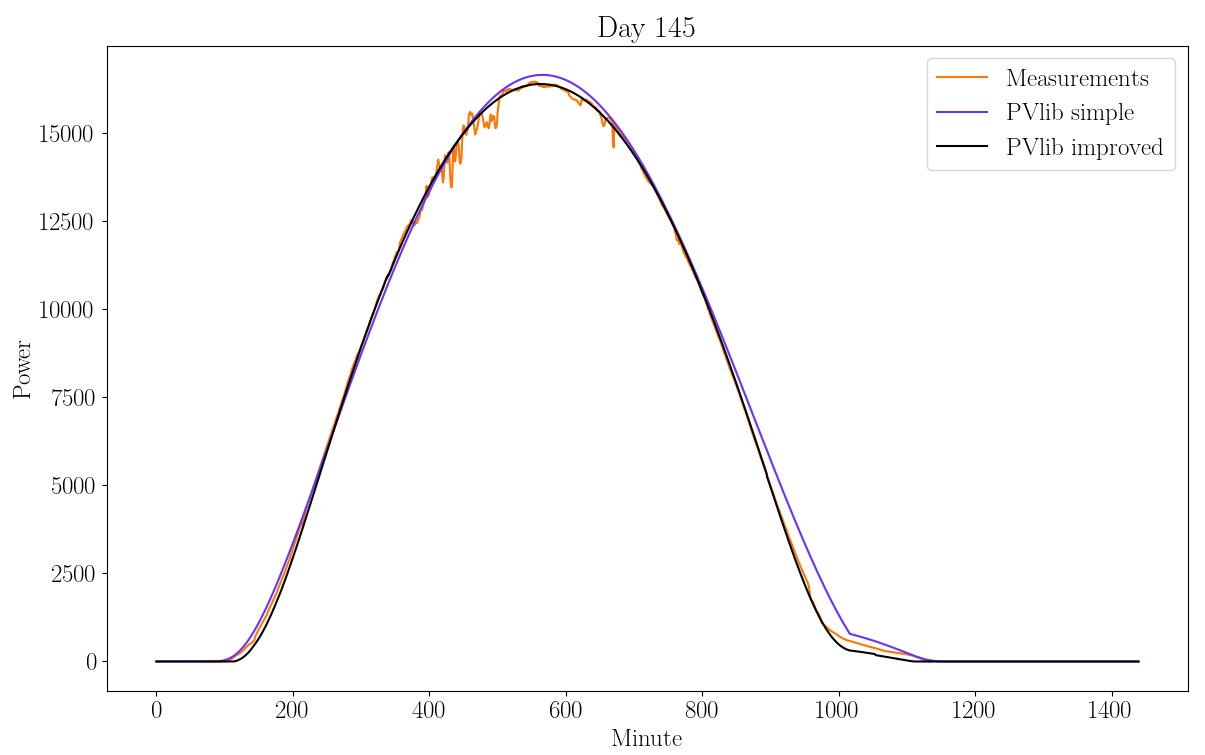
\includegraphics[width=0.99\linewidth]{pics/pvlibsimplecomplex}
\figcaption{Comparison of PVlib POA and the improved PV power generation model on a day from Helsinki dataset.}
\label{fig-poa_eval_simplecomplex}
\end{figure}

\noindent Figure \ref{fig-poa_eval_simplecomplex} shows what the improvement looks like in a best case scenario. The improved model can be seen to approximate the power output with comparable or higher accuracy than the POA model during a modeled day. Despite the good performance of the improved model, the POA model still has uses due to faster computational speed. If for example only the first and last non-zero minutes matter, it may not make sense to use a physically more accurate model. In the next chapters which of these models is being used will be mentioned on case by case basis.



%that the improved PV model performs better than the simple POA-model at 1000 minutes where the AOI is high and thus reflective losses from direct irradiance are significant. And during peak production minutes where the panel temperatures are likely high enough to cause thermal losses.

%The improved model would appear to be a more accurate approximation for PV generation than the POA model, but the POA model still has uses in applications where faster computation is beneficial or where only the timing of the first and last non-zero minutes matter. Which of these models is being used will be mentioned in the following chapters.

%The model performance could be further tuned as inverter efficiency and other possible factors were not taken into account. However as there are only two datasets, this would increase the likelyhood of overfitting and thus the improved model is left as is.


%is near 90$^\circ$ and during peak production hours where increased temperature effects performance. This is promising but the complexcity of the model also increases the likelyhood of overfitting. Nevertheless this improved model with 2m/s wind speed, 8m elevation and 25 $^\circ$C ambient temperature and the POA model will both be used in the following chapters depending on the charasteristics of parameter estimation functions.

%\noindent Figure \ref{fig-poa_eval_single_day} show that simulations are fairly accurate but there seems to be some deviations between the simulated values and the measurements. The two significant deviations are the noise during peak power generation period and the smooth decrease in power generation during the last hours of the day. The peak power generation noise is likely to be caused by decreases in efficiency due to heat the occasional cooling from gusts of wind. The second deviation between the model and actual measurements is likely to be caused by panel reflections as the south-east orientation of the solar panels results in a high angle of incidence during the last hours of the day.

%Modeling these physical phenomena is possible to an extent if the components of plane of array irradiance are used instead of the POA values. As per Sandia National Laboratories \cite{sandia_poa}, the three components of plane of array irradiance are direct normal irradiance(DNI), global horizontal irradiance(GHI) and diffuse horizontal irradiance DHI. A physically accurate model would compute the absorbed radiation by first projecting the irradiance components to the plane of array adn the estimating the losses caused by reflections. After this is accomplished, the absorbed irradiance could be used to estimate panel temperature and power output.








